% Williams Physics Thesis template
% Patterned after the work of Cole Meisenhelder '15
% Commented by Prof. Charlie Doret, 12/2016
% Uploaded to Overleaf by Dr. Kevin Flaherty, 5/2021

\documentclass[12pt, oneside]{book} 

% The \usepackage{} command will import predefined fonts, symbols, environments, etc.  For example, the ams packages below come from the American Mathematical Society and include all kinds of useful math symbols like integrals
\usepackage [english]{babel}
\usepackage [autostyle, english = american]{csquotes}
\MakeOuterQuote{"}

\usepackage{amscd}
\usepackage{amsmath}
\usepackage{amssymb}
\usepackage{amsthm}
\usepackage{verbatim}
\usepackage[utf8]{inputenc}
\usepackage{geometry}                		% See geometry.pdf to learn the layout options. There are lots.
\geometry{letterpaper}                   		% ... or a4paper or a5paper or ... 
%\geometry{landscape}                		% Activate for for rotated page geometry
\usepackage[pdftex]{graphicx}				% Use pdf, png, jpg, or eps� with pdflatex; use eps in DVI mode	
\usepackage{setspace}
\usepackage{physics}
\usepackage{subcaption}
\usepackage{natbib}
\usepackage{pdfpages}
\usepackage{bm}
\usepackage{wrapfig}				% enables the use of \wrapfig, for figures with text wrapped around them
%\usepackage{lipsum}			% gives access to \lipsum, which dumps some latin text into your document as filler if you want to check formatting

%\usepackage[parfill]{parskip}    		% Activate to begin paragraphs with an empty line rather than an indent


\setcitestyle{authoryear,open={(},close={)}}

% Here we set the page dimensions to match the standard thesis format.  These values should not be changed.
%%% SET LENTGH AND WIDTH %%%
\setlength{\textwidth}{6.5in}
\setlength{\textheight}{8.5in}
\setlength{\oddsidemargin}{0pt}
\setlength{\evensidemargin}{0pt}
\setlength{\topmargin}{0pt}
\setlength{\marginparsep}{0pt}
\setlength{\marginparwidth}{1in}



% DEFINITIONS
\def \lcdm {$\Lambda$CDM}


%\begin{document} starts LaTeX looking for actual content.  Everything above this point is purely formatting.
\begin{document}

\begin{titlepage}
\begin{center}

% \vspace* creates some vertical white space on the page to make the title page look more pleasing.  \vspace would do much the same thing, but would not insert the white space if we were at the top of a fresh page.  As this is the start of the document we're obviously at the beginning of a page, so the asterisk is necessary to ensure we still put in two cm of white space.
\vspace*{2cm}

{\huge Large Ultra-Faint Galaxies in the Firebox Simulation} % \huge sets the font size.  Other options include things like \large, \Large, \small, \tiny, etc.

\vspace{2cm}

{\large by\\Marckie Zeender}

\vspace{2cm}
{Professor Moreno, Advisor}

% \vfill creates an arbitrary amount of vertical white space as necessary to fill the page
\vfill

A thesis submitted in partial fulfillment\\
of the requirements for the\\
Degree of Bachelor of Arts with Honors\\
in Physics

\vspace*{3cm}

Pomona College\\
Claremont, California\\
\today % you might choose to set a permanent date, but \today will put in today's date
\end{center}
\end{titlepage}

% \frontmatter defines the pieces of the thesis which will use roman numerals for page numbering
\frontmatter 


% \chapter{} and/or \chapter*{} will create a chapter in your thesis.  Including the asterisk will cause the chapter to not appear in the table of contents.

% \input will reference a particular .tex file.  Here we are grabbing a file entitled Abstract stored in the folder Chapters
\chapter{Abstract}
\input{Chapters/Abstract}
\chapter{Executive Summary}
% Here we have your executive summary.

Cosmological simulations are an important part of our understanding of the universe. They allow us to test our theories about cosmology by seeing if the simulated behavior created by those theories aligns with the real world. The FIREbox galaxy simulation uses the theory of \textbf{\lcdm}, the current most popular model of dark matter and dark energy. FIREbox models a universe of over 1700 galaxies from their initial creation all the way through the present day. This present state can be compared to real-world galaxies to determine what simulated characteristics align with the real ones.

When a certain characteristic of the simulation does not line up with observational data, it is called a \textbf{tension}. One such tension is that of the diversity of low-mass galaxy sizes. The low-mass galaxies near the Milky Way (known as the \textbf{Local Group}) have much variation in radius compared to their mass. In other words, they range from very compact to very fluffy. However, most historical \emph{simulated} galaxies have a much stricter size-mass ratio. This discrepancy is the driving motivation for this thesis.

To examine the tension further, I compare the fluffiness of galaxies from the FIREbox cosmological simulation with other galactic properties. I define the \textbf{fluffiness} ($\beta$) of a galaxy to be how much it deviates from the expected size-mass ratio. This parameter is useful for our study because, by design, it is independent of mass for low-mass galaxies. We are therefore free to correlate it with other parameters.

One theory for this tension is tidal disruption. Tidal disruption occurs when a galaxy comes in close contact with another, and its outer layers get stretched by the other's gravity. Tidal forces might therefore increase fluffiness. I tested this by examining the relationship between a satellite and its host galaxy (satellites are galaxies that orbit other galaxies). I compared the fluffiness of satellite galaxies with the distance to their hosts: both in the present and when they were at their \emph{minimum} distance. I found that when you express the distance as a fraction of the host galaxy's virial radius, there is a correlation. In other words, the closer a satellite gets to its host, the more fluffy it becomes.

\chapter{Acknowledgments}
% Here we have a section where you might choose to acknowledge your family, fellow students, advisor, dog, etc.

To Profe Moreno for reading my draft %TODO: change this

%\tableofcontents will create a table of contents.  By default it will include entries for any \chapter, \section, and \subsection command that appears in your thesis unless you have called the tag with an asterisk
\tableofcontents

\listoffigures

% \mainmatter defines the main body of the thesis and marks where regular numbering will begin
\mainmatter

\chapter{Introduction}
% Look!  A mock introduction
Understanding the composition and structure of galaxies and the role that dark matter plays in their organization is one of the most pressing topics in modern intergalactic physics. A common method to explore these questions is using simulations. A simulation allows us to choose plausible initial conditions and plausible laws of physics and test how the universe would behave under those conditions. We can then compare those results to experimental data to examine the accuracy of those initial assumptions.

\section{FIREbox Galaxy Simulation}
The FIREbox (\cite{feldmann_firebox_2022}) simulation is the most in-depth galaxy simulation ever performed as of the date of this thesis. It does not have the largest volume, nor is it the most detailed; sub-simulations such as FIRE in the Field (\cite{fitts_fire_2017}) zoom in closer, to a particle size as low as 500 solar masses. FIREbox, however, has the total combined resolution and incorporates a balance of detail and scale.




\section{FIREbox Galaxy and Halo catalog}
Over the course of the simulated universe's evolution, 1201 snapshots of the state of the universe were collected (\cite{feldmann_firebox_2022}). They were approximately evenly spaced out in time and included the positions of the particles, their densities, metalicities, star-formation rates, and other properties. The particle data was reduced by grouping the particles into their respective galaxies and dark matter halos. They used the AMIGA Halo Finder (AHF; \cite{knollmann_ahf_2009} to sort the halos into categories of halos and sub-halos, which in turn allowed them to categorize the galaxies by host and satellite galaxies respectively. The reduced data, known as the galaxy and halo catalog includes galaxy information such as CM position, radius (measured using 

AAAAAAAAAAAAAAAAAAAAAAAAAAAAAAAA

The introduction is one of the most important pieces of your thesis.  Here is a place for you to introduce the problem(s) on which you have worked and place them in the larger context of your field.  You should aim to ensure that this section is completely understandable to virtually anyone - and certainly anyone with a sophomore-level grasp of physics.  Presumably this will include references to the literature.

In addition to setting your work into context, a second good idea for your introduction is to give a short outline for what the rest of your thesis will discuss.  This is often done in the closing paragraph(s) of the introduction with sentences like ``In the following chapters \ldots " and ``Chapter 2 discusses \ldots"  Tremendous detail is not required in this outline, but rather just a brief road map for the rest of the document.

\section{Oh}

\section{Another section}

This second section is, obviously, 1.2.

\subsection{A subsection}

\subsubsection{A subsubsection}

Subsubsections are still smaller sections.  By default, this is the finest subdivision of a chapter in \LaTeX, and they will \emph{not} appear in the table of contents.  

\subsection{A useful command}

\marginpar{This is a margin note.}
One command I often ask my students to use is \texttt{\textbackslash marginpar}, which can be used to create a margin note.  These are super helfpul if there's something to which you need to return later (say, after you've looked up a number), as notes in the margin are really easy to find quickly.  

\section{Some figures}

You will surely want to add figures to your thesis to help explain your ideas.  There are a number of different ways to include such things, but the most typical way would be to generate the figure in another piece of software (\texttt{MATLAB, Mathematica, Adobe Illustrator, \ldots} and simply include it in your \LaTeX ~code.  This will require use of the \emph{figure} environment.\footnote{there are many other possible environments to include figures, such as wrapfigure, but these will require including additional packages \ldots}  See this document's \LaTeX ~code for details . . .

% Here is the figure environment.  The [] after \begin{figure} are an optional argument that tells LaTeX where to try to place the figure.  If you do not include it then it will figure out the `best' place to put things on its own, but on occasion the choices it makes are a bit strange.  Even so, you should probably try to let it make the decisions whenever possible, and only come back to enforce new locations after you have essentially finished your document.  Otherwise you may find that your instructions are no longer appropriate if you add text elsewhere in the document that changes how things are alligned.  Anyhow, [h] instructs LaTeX to put th e figure `here', and adding an exclamation point [h!] means REALLY, PUT IT HERE.  [t] and [b] mean to put the figure at the top or bottom of a page, respectively.
\begin{figure}[ht!]

%\centering centers the figure on the page.  This is convention.
\centering

% The \includegraphics command is the default way to include a figure.  The first optional argument in [] brackets defines how large the figure should be on the page.  This can be defined in inches, centimeters, or as a fraction of the \textwidth.  Then, in the curly {} braces you will put the file name for the figure.  Here it has been stored in a subfolder entitled Figures.  You are encouraged to give your figures descriptive file names, as this will help future students to figure out what figure corresponds to which file without having to read your LaTeX code.  

%\caption will create a figure caption.  Putting an asterisk after it (as in \caption* ) will cause the caption to not be numbered and to not appear in the list of figures.  The [] argument is optional but recommended; this is the short-form caption which will appear in the list of figures.  The {} argument is required, and gives the full caption which will appear in the main text.  The first few words of this caption will be used in the list of figures if no [] form is given.  
\caption[Short-form caption]{Long-form caption that appears in main body of the document}

% the \label gives a reference for this figure so that you can refer to it in the text by its number in a way which will be automatically updated if you change the document.  THIS IS A GOOD IDEA; having automatically updated references for figures, equations, etc, will keep your document in order even as you continue to update it over a period of months.  This reference can be called in the text using the \ref tag.
\label{fig:aFigure}
\end{figure}



Here, back in the main body of the text, we can create a reference to figure \ref{fig:aFigure}.  This is automatic; the actual numbers are not typed into the code, but rather the \texttt{\textbackslash ref} tag has been used.  Always always always use the \texttt{\textbackslash ref} command to reference figures, or invariably at some point you'll move something and all of your references will be incorrect and you'll have to fix them manually.

% Here is the same figure, but now using the wrapfigure environment.  This allows you to wrap your text around the figure itself.  The optional [] argument specifies how many lines of text should be wrapped.  The first {} argument specifies where on the page the figure should live (here the right side is specified).  The second {} argument defines how much real estate on the page will be allocated for the figure block; here it is 45% of the page width.
\begin{wrapfigure}[11]{r}{0.45\textwidth}
\centering
% \vspace creates vertical white space in the document.  Here we are creating 0.1 lines of text worth of negative white space, effectively moving our graphic up in the document by one line.  I find this lines things up better within the text in this case, but you may need to manipulate this to make the alignments look correct.
\vspace{-.1\baselineskip}
\caption[Another short-form caption]{A figure included using the wrapfig environment}
\label{fig:anotherFigure}
\end{wrapfigure}
As an alternative to the ordinary figure environment, you might deem it desirable to tuck a figure in more closely amongst the text.  This has a separate environment known as \emph{wrapfig}.  Here we will include the same figure as above a second time, but this time using the \emph{wrapfig} environment.  This will insert the figure into your document with the text wrapping around the perimeter, rather than offsetting it into its own separate chunk of page, as above.    As before, we can use an automated reference to the figure using the \texttt{\textbackslash ref} tag; here we have figure~\ref{fig:anotherFigure}.  Working with the wrapfigure environment sometimes requires a little bit of massaging to ensure that everything lines up properly in your document, but with a small amount of work  you will find that you can get the text to box the figure quite nicely.

Here I have added a table, because tables are also useful. This table has nothing to do with the rest of the material in this thesis template, but you should probably only add relevant tables.
\begin{table}[tbh]
\begin{center}
%\caption[]{\em{Here we show the continuum sensitivity required per band.}}
\begin{tabular}{ccccccc}
\hline \noalign {\smallskip}
Name & SpT & Dist. & Age & 3$\sigma$ M$_{\rm dust}$ & 3$\sigma$ CO(3-2) limit & Disk indicator \\
 & & (pc) & (Myr) & limit (M$_{\oplus}$) &  (mJy km s$^{-1}$)\\
\hline \noalign {\smallskip}
J0226 & L0 & 46.5 & 45 & 0.01 & 24 & Pa$\beta$, IR\\
J0501 & M4.5 & 47.8 & 42 & 0.01 & 23 & H$\alpha$, IR\\
J1546 & M5 & 59.2 & 55 & 0.01 & 14 & HeI, [OI], H$\alpha$, IR\\
J0446 A/B & M6/M6 & 82.6/82.2 & 42 &  0.027 & 18 & H$\alpha$, IR\\
J0949 A/B & M4/M5 & 79.2/78.1 & 45 &  0.024 & 17 & H$\alpha$, IR\\
LDS 5606 A/B & M5/M5 & 84/84 & 30-44 & 0.027 & 19 & H$\alpha$, IR, UV\\
\hline \noalign {\smallskip}
\end{tabular}
\end{center}
\end{table}




\chapter{Methods}
\section{FIREbox: a novel cosmological simulation}
Scale and resolution are important for simulations. Astrophysicists must balance large volume and high detail, both of which cost computing power. The large volume simulations allow us to closely study intergalactic systems and to collect large amounts of statistical information about galaxies \citep{feldmannFIREboxSimulatingGalaxies2022}. However, a higher resolution "zoom in" simulation such as FIRE in the Field \citep{fittsFireFieldSimulating2017} allows us to better simulate the internal physics of the galaxies themselves.

This paper will examine data from FIREbox \citep{feldmannFIREboxSimulatingGalaxies2022}. This cosmological simulation does not have the largest volume, nor is it the most detailed. Rather, it incorporates a balance of high detail and large scale (see Figure \ref{fig:feldmann-dynrange}), which together give it the highest dynamical range of any cosmological simulation to this date.

\begin{figure}
    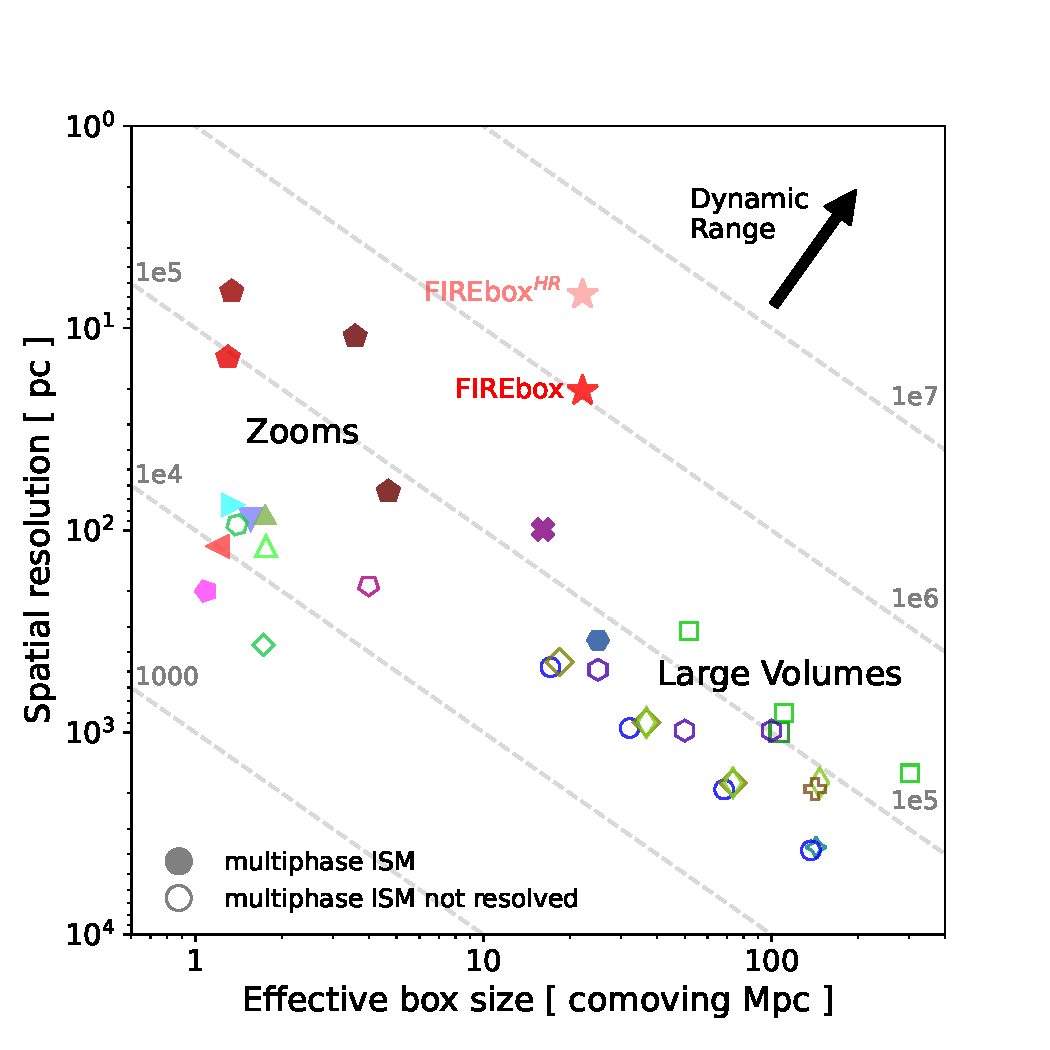
\includegraphics[width=\textwidth/2]{figs/feldmann/fig2a}
    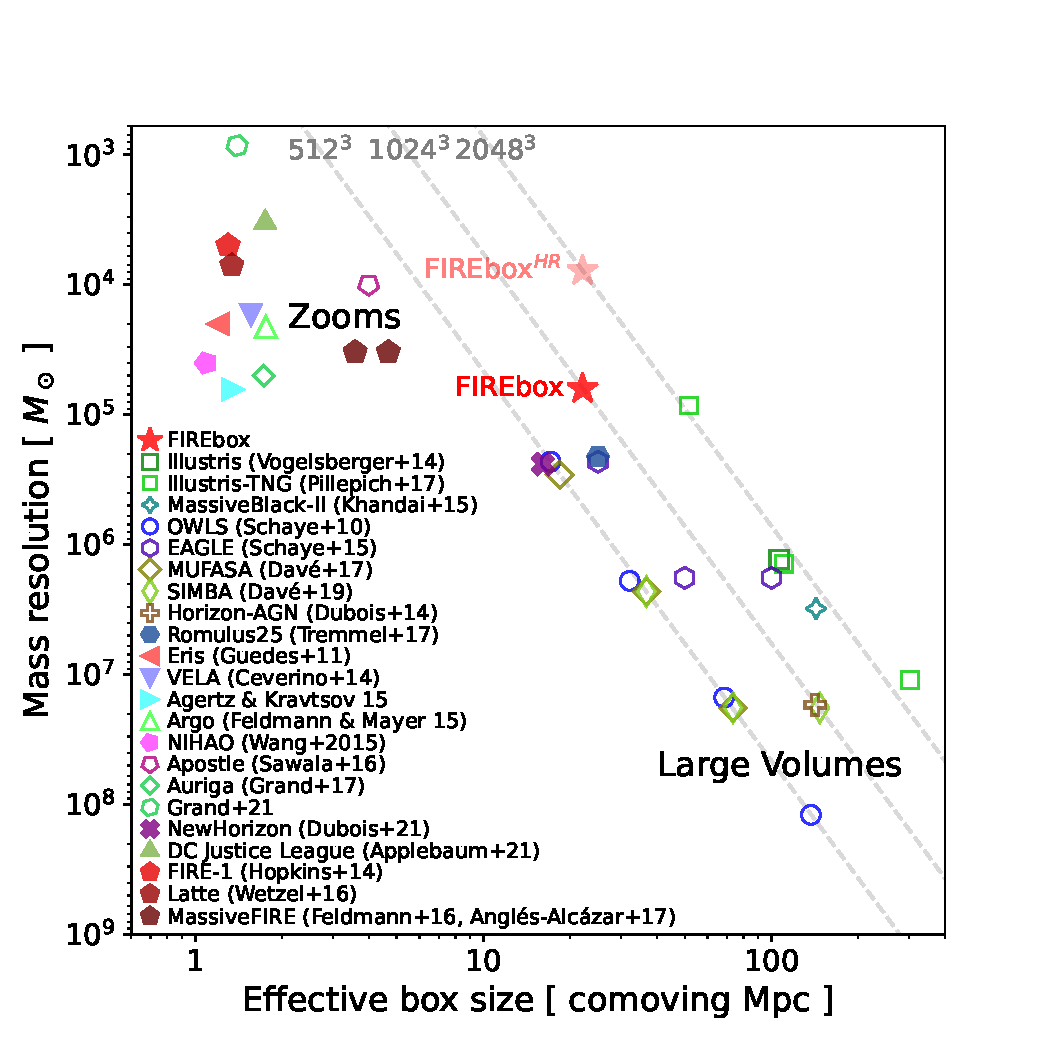
\includegraphics[width=\textwidth/2]{figs/feldmann/fig2b}
    
    \caption{A comparison the size and detail of cosmological simulations. There is a tradeoff between scale and resolution, where a total increase in both means a higher dynamic range at the cost of computer performance. FIREbox has the highest dynamic range, and therefore the highest computational cost.}

    \label{fig:feldmann-dynrange}
\end{figure}

\section{The data}
Over the course of the evolution of the FIREbox simulation, 1201 snapshots describing the state of the universe were collected \citep{feldmannFIREboxSimulatingGalaxies2022}. They were approximately evenly spaced out in time and included the positions of the particles, their densities, metallicities, star-formation rates, and other properties. The particle data was reduced by grouping the particles into their respective galaxies and dark matter halos. The authors used the AMIGA Halo Finder \citep[AHF;][]{knollmannAhfAMIGAHALO2009} to sort the halos into two hierarchical categories: main halos and sub-halos. This, in turn, allowed them to categorize the galaxies by hosts and satellites, respectively. The reduced data, known as the galaxy and halo catalog, includes galaxy information such as position, radius, mass and star formation rate, as well as data about the dark matter halos around those galaxies. I will be mostly using snapshot 1201, the final state of the simulation. This snapshot depicts the simulated present day.

Each parameter for the galaxies is split between a few different definitions. For the purpose of this thesis, I will use the following definitions unless otherwise specified. The galaxy's radius $R_{50}$ is defined to be the radius containing 50\% of its stellar mass, as determined by AHF. The galaxy's mass $M_\star$ is defined to be the mass of the stars contained within $R_{50}$. I will not include dark matter in this definition. The reader should note that this is not the only way to define these parameters. Due to the fluid nature of matter on a galactic scale, it is often arbitrary as to whether a given particle belongs to a given galaxy. Alternate definitions include different thresholds for the radius, such as $R_{80}$, and different kinds of matter included in the mass, such as gas matter and dark matter.

Other parameters that I will use are a galaxy's position in space and its flyby distance---a satellite galaxy's minimum distance to its host galaxy. All distances (including radius) are measured in terms of the co-moving parameter $h$, a time-dependent scaling factor of the universe. In the final state of FIREbox, $h = 0.6774 \text{ kpc}$. 

\cite{mcconnachieOBSERVEDPROPERTIESDWARF2012} compiled a number of data sets for low-mass galaxies in the Local Group. One data set includes the galaxies' radii and another contains their masses. The radius is defined slightly differently in this case. It is the half-light radius, the radius from which half of the galaxy's light is emitted.
Klein et al. (in prep) shows that the half-light radius is functionally identical to $R_{50}$. $M_\star$ is calculated by assuming a mass-light ratio of one, meaning that the brightness per unit mass is equal to the Sun.

To get this data in a usable form, I first dumped the text-based datasets into pandas spreadsheets and removed rows with missing data. I then merged the datasets by galaxy name. For galaxies whose names were reported differently on the different sheets, I merged them by hand. I then cast the mass and radius to float64 for use in the analysis.

% TODO: discuss figs 2.1 and 2.2 earlier

\begin{figure}
    \includegraphics*[width=\textwidth]{figs/feldmann/fig1.pdf}
    \label{fig:feldmann-visual}
    \caption{
        From: \cite{feldmannFIREboxSimulatingGalaxies2022}. A representation of the FIREbox simulation. The first two rows depict the state of the simulation at three different time points; the rightmost images depict the simulation in the present time. The top row depicts dark matter in blue and stellar matter in white, while the middle row depicts gas. The bottom row shows a galaxy at different scales. As one can see, matter collects into galaxies and systems of galaxies over the course of the simulated universe's evolution. These galaxies take on a variety of sizes, and they share threads of gas and are contained within hierarchical halos of dark matter.
    }
\end{figure}

\begin{figure}
    \centering
    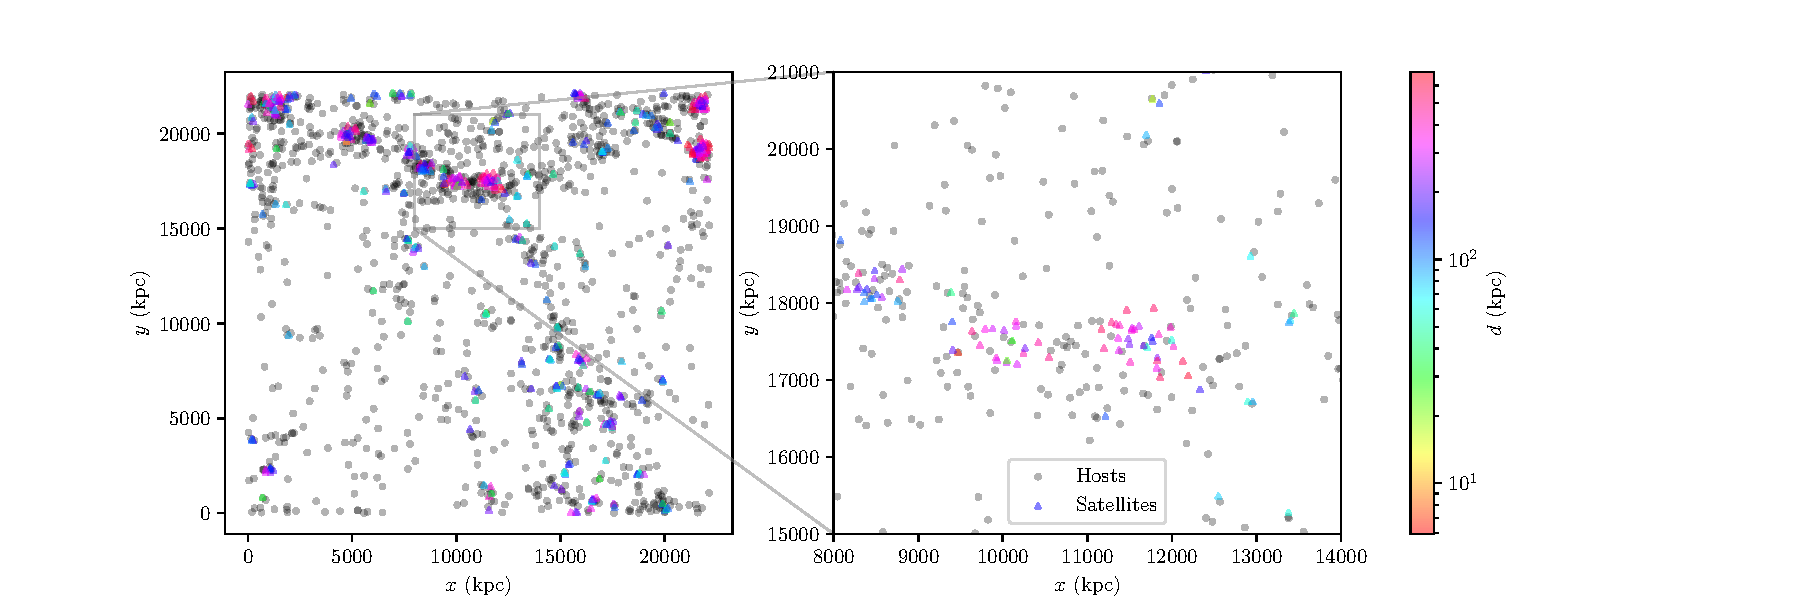
\includegraphics[width=\textwidth*11/10]{figs/me/locations.pdf}
    \caption*{
        A 2D visualization of FIREbox; the X and Y coordinates of each galaxy. Host galaxies are depicted as gray circles, and satellites galaxies are triangles that are colored by the distance to their host galaxy. 
    }
\end{figure}

\begin{figure}
    \centering
    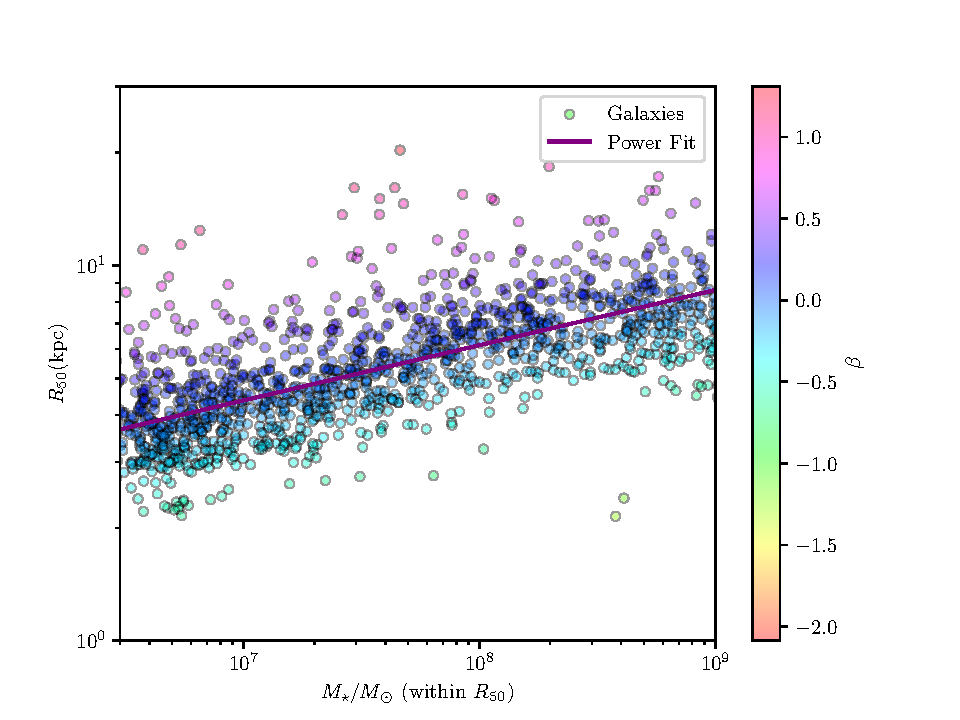
\includegraphics[width=\textwidth*2/3]{figs/me/stars-mass-size-r50.pdf}
    \caption{
        The left shows the size-mass relationship for the FIREbox low-mass galaxies. It covers the range $3 \times 10^3$ -- $1 \times 10^9 M_\odot$. Galaxies larger than this are no longer dwarfs and do not follow the power law, and galaxies smaller than this approach FIREbox's resolution limit. The line of best fit is described by equation (\ref{equ:linear-rel}) and $\beta$ represents the deviation from that line. $\beta$ is chosen to characterize the diffuseness of a galaxy because the distribution of $\beta$ is independent of mass for low-mass galaxies (see Figure \ref{fig:beta-mass}).
    }
    \label{fig:size-mass}
\end{figure}

\section{The Diffuseness Parameter}
As diffuseness will be main subject of this paper, let us define it. The low-mass galaxies in FIREbox loosely follow a power law size-mass relationship (see Figure \ref{fig:size-mass}). The relationship can therefore be described using the following equation,
\begin{equation}
    \frac{R_{50}}{1 kpc} \approx a
    \left(
        \frac{M_\star}{M_\odot}
    \right)
    ^{\gamma}
\end{equation}
where $\gamma$ and $a$ are constants and $M_\odot$ is the mass of the sun. I am dividing by a kiloparsec unit to make the equation unitless. Taking the logarithm of this equation yields
\begin{equation}
    \label{equ:linear-rel}
    \ln \left(
        \frac{R_{50}}{1 \text{ kpc}}
    \right)
    \approx
    \ln(a)
    + \gamma \ln \left(
        \frac{M_\star}{M_\odot}
    \right)
\end{equation}

By taking the natural logarithm of a power law, I end up with an equation for a line. This linear relationship can be seen in Figure \ref{fig:size-mass}. Here, $ln(a)$ becomes the $y$-intercept of the line and $\gamma$ becomes the slope. I have kept denoting this equation as \emph{approximately} equal in order to emphasize that not every galaxy falls exactly into this relationship. However, one can replace that by introducing a galaxy-specific parameter $\beta$ that is defined to be the galaxy's deviation from this linear relationship:
\begin{equation}
    \label{equ:log-log-with-beta}
    \ln \left(
        \frac{R_{50}}{1 kpc}
    \right)
    =
    \ln(a)
    + \gamma \ln \left(
        \frac{M_\star}{M_\odot}
    \right)
    + \beta
\end{equation} 

\begin{equation}
    \label{equ:beta}
    \beta
    \equiv
    \ln \left(
        \frac{R_{50}}{1 kpc}
    \right)
    -
    \ln(a)
    - \gamma \ln \left(
        \frac{M_\star}{M_\odot}
    \right)
\end{equation} 

I will call $\beta$ the \textbf{diffuseness parameter}, because it tells us how diffuse a galaxy is relative to its fellow galaxies. Positive values of $\beta$ mean that the galaxy has a larger radius than other galaxies of the same mass, and negative values mean a smaller radius. $\beta$ is especially useful for characterizing the diffuseness because the distribution of $\beta$ remains consistent across all masses of low-mass galaxies (see Figure \ref{fig:size-mass}). Note that this does not apply to galaxies larger than $10^9 M_\odot$ (see Figure \ref{fig:beta-mass}).


$\gamma$ and $\ln(a)$ are calculated using equation (\ref{equ:linear-rel}) and fitting the dataset to a line. One can then use those values in equation (\ref{equ:beta}) to find each galaxy's value of $\beta$. One can also characterize the \textbf{diversity of the diffuseness} of galaxies using the the standard deviation $\sigma_\beta$ (the mean is zero by design). I will use these values to compare FIREbox with the galaxies of the Local Group.

\begin{figure}
    \centering
    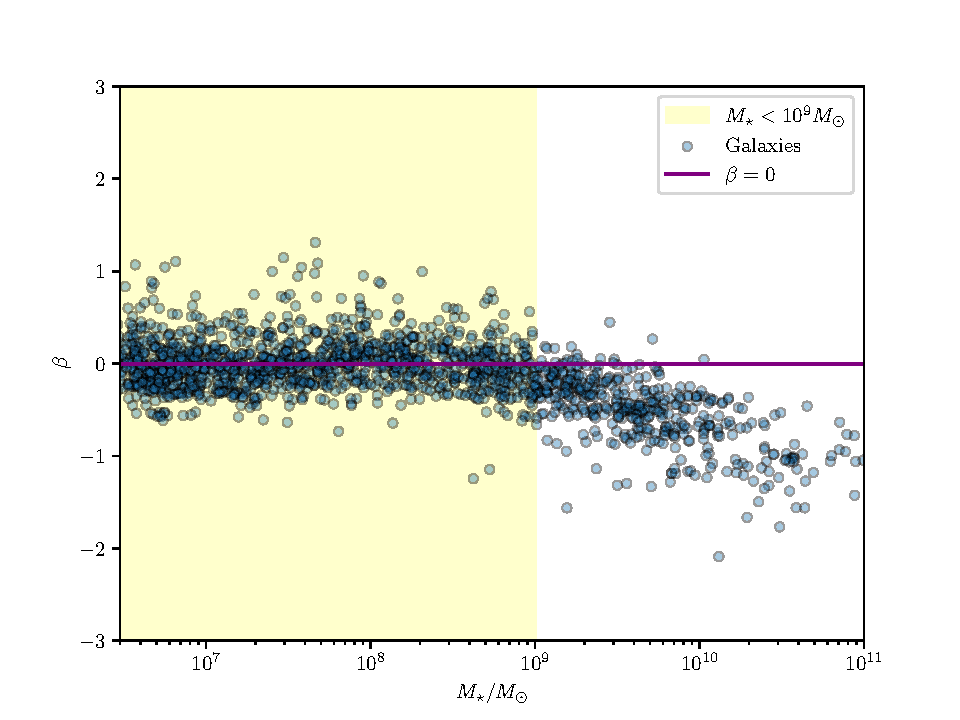
\includegraphics[width=\textwidth*2/3]{figs/me/beta-mass.pdf}
    \caption{The relationship between $\beta$ and mass. The distribution of $\beta$ is independent of mass for the low-mass galaxies I will examine in this thesis.}
    \label{fig:beta-mass}
\end{figure}

\section{Proximity}


 Tidal disruption may provide an explanation for diffuseness. Tidal forces are caused by a gradient in the gravitational field, that causes objects to be stretched. I inspected FIREbox galaxies' tidal interactions with their neighbors. Specifically, I examined a galaxy's distance to its nearest neighbor, as well as a satellite galaxy's distance to its host galaxy. For the distance to the host galaxy, I examined both the absolute separation and virial separation. I define the absolute separation to be the distance in kpc to the host galaxy, and the virial separation to be that distance as a fraction of the host galaxy's virial radius. The virial radius of a galaxy is the radius within which particles will tend to be gravitationally bound. In other words, it is the effective radius of a galaxy's gravitational well.

 \cite{jacksonDarkmatterdeficientDwarfGalaxies2021} defines the "perturbation index" (PI), which characterizes the strength of the tidal effect on an object in a virial halo. The PI is proportional to the inverse of the virial separation cubed. This power relationship means that we can test for tidal disruption using the virial separation.

 \subsection{Minimum Proximity}

 To determine whether tidal interactions affect the diffuseness of galaxies, it may be better to consider the \emph{minimum} distance between a satellite and its host, as opposed to the current distance. The minimum distance is the point at which the tidal forces are strongest, and therefore could cause the most extreme effects. I will therefore also compare $\beta$ to $d_{\rm{min}}$, using both the absolute and virial separation. Note that such an analysis is only possible with simulation data because we can only view the real universe in its present state. This analysis will exclude satellites that have not reached the perihelion of their trajectory.

\subsection{Calculating distances}

Calculating the distance between two galaxies in FIREbox is not as trivial as it may seem. The simulation volume is defined as a cube that repeats itself \citep{feldmannFIREboxSimulatingGalaxies2022}. In other words, if you travel across one border of the universe, you appear on the opposite side. This geometry is adopted to avoid any strange boundary conditions---it would be unrealistic for there to by enormous walls in space, for example. However, it is also impossible to simulate an infinite universe. This "wrapping around" model allows for a middle ground.

In order to measure the $x$ component of the distance between two objects one must first determine whether they are across the $x$ border. If they are, then one find the sum of the distances to the border. Otherwise, one finds the difference of their positions like normal. The same logic is used to find the $y$ and $z$ components. Only then does one calculate magnitude of the distance. Refer to Appendix \ref{apx:distances} for code to do this calculation.




% the \appendix tag tells LaTeX where it should start labeling chapters with letters (denoting appendices) rather than numbers (denoting main chapters)
\appendix 


\chapter{An appendix}
% Look!  An Appendix!

\chapter{Calculating distances in FIREbox}
\label{apx:distances}
The following code finds the distance to the closest galaxy. Note that for each coordinate, one must check whether the separation is greater than 7500, implying that the distance should be measured across the border.

\begin{lstlisting}[language=Python]
def get_nearest(row):
    
    r = np.array([
        row.Xc_ahf_cat, row.Yc_ahf_cat, row.Zc_ahf_cat
    ]).reshape((1, 3))
    
    r_other: np.ndarray = dat.loc[:, (
        'Xc_ahf_cat', 'Yc_ahf_cat', 'Zc_ahf_cat'
    )].to_numpy(dtype='float64')
    
    # 2d array: each row contains the x, y, z separation
    delta_r_vec = r_other - r
    
    # whether the coordinate is across the border
    is_over = delta_r_vec > 7500
    
    # if across the border, subtract delta_r from 15000
    delta_r_wrapped = (15000 - delta_r_vec) * is_over
    
    # else, use delta_r as is.
    delta_r_wrapped += delta_r_vec * ~is_over
    
    # find the magnitude
    delta_r_mag = np.sqrt((delta_r_wrapped**2).sum(axis=1))
    
    # set the distance to oneself to an arbitrary
    # large number (to exclude it from the calculation)
    delta_r_mag += 15000 *(delta_r_mag == 0.0)
    
    nearest_galaxy = (
        dat['galaxyID']
        .to_numpy(dtype=int)[delta_r_mag.argmin()]
    )
    
    prox_to_nearest = delta_r_mag.min()
    
    return pd.Series(
        dict(
            galaxyID=row.galaxyID,
            nearest_galaxy=nearest_galaxy,
            d_comoving=prox_to_nearest,
            
            rvir_nearest=dat['Rvir_ahf_cat'].to_numpy(
                    dtype='float64'
                )[delta_r_mag.argmin()]
        )
    )

    
\end{lstlisting}



% \bibliographystyle tells LaTeX how you want to format your bibliography.  There are many standard formats.  apsrev is fairly typical, but feel free to explore other options if the mood strikes.  
\bibliographystyle{apsrev}

% \bibliography calls the actual file that contains your bibliographic information.  This file can be generated by hand or in an automated way using software such as BibTeX.  Either works fine, but it is worth learning to use BibTex in the long term.  Take a look at the .bib file included here if you want to get some idea of the formatting required to create a bibliogrphy file of your own.

\bibliography{references}
\end{document}